\section{正则性}
\label{sec:ellip-regularity}

Lax--Milgram定理给出的弱解只在$H^1$中。它是否具有更好的性质，比如二阶导数平方可积、逐点连续，甚至光滑？这决定了弱解是否就是经典解，也决定了数值方法能达到多高的精度。答案取决于系数、源项和区域三者，而且内部和边界的情况不一样。

\paragraph{一维的情形}
在一维可以直接看到。$-u''=f$的弱解满足$u''=-f$，所以$f\in L^2$时$u\in H^2$，$f$连续时$u\in C^2$，一般地$f\in C^k$时$u\in C^{k+2}$。解比源项多两阶导数，这正是“两次积分”的效果。

图~\ref{fig:ellip-regularity-ladder}取跳跃的源项$f=\mathbf{1}_{(1/2,1)}$，零边界。解$u$的二阶导数就是$-f$，有跳跃，所以$u\in H^2$但$u\notin C^2$。$u'$连续但有折角，$u$是$C^1$的，已经看不出任何异常。

\begin{BookInlineFigure}
  \centering
  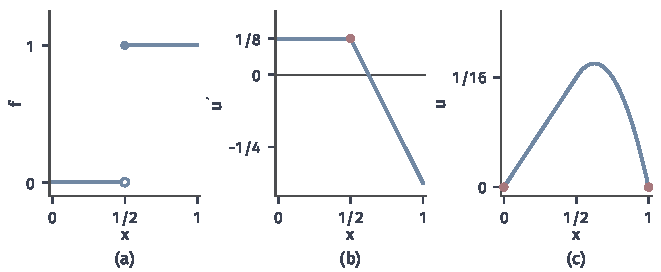
\includegraphics[width=112mm]{figures/06-differential-equations/02-partial-differential-equations/matplotlib/ellip-regularity-ladder/figure.pdf}
  \caption{解比源项多两阶光滑性。(a)源项$f$在$x=1/2$处跳跃。(b)$u'$连续，在红点处有折角。(c)$u$是$C^1$的，曲线在中点看不出异常。由式~\eqref{eq:ellip-interval-solution}，$x\leq1/2$时$u=x/8$，$x\geq1/2$时$u=1/16+(x-\tfrac12)/8-(x-\tfrac12)^2/2$。}
  \label{fig:ellip-regularity-ladder}
\end{BookInlineFigure}

这种增益来自源项，前提是系数足够好。图~\ref{fig:ellip-coefficient-jump}的两段材料中，$f=1$是光滑的，解在界面处却有折角，$u'$有跳跃，$u\notin H^2$。方程能保证的是通量$au'$在$H^1$中，而把$a$除掉后，$u'$的光滑性不会比$a$好。这说明系数必须有一定的光滑性才能得到$H^2$。

\paragraph{为什么Laplace算子能控制全部二阶导数}
多维的情形有一个疑问：方程只给出了$\Delta u$，即二阶导数的一个特定组合，它凭什么控制全部的二阶导数？对$v\in C_c^\infty(\mathbb{R}^{d})$，分部积分两次，
\[
 \int\partial_i\partial_jv\,\partial_i\partial_jv\,\mathrm{d}\bm{x}=\int\partial_i\partial_iv\,\partial_j\partial_jv\,\mathrm{d}\bm{x}.
\]
对$i,j$求和，得到恒等式
\begin{equation}
 \lVert\nabla^2v\rVert_2=\lVert\Delta v\rVert_2 .
 \label{eq:ellip-hessian-identity}
\end{equation}
Hessian的全部元素的平方和，积分后恰好等于$\Delta v$的平方的积分。这个恒等式是椭圆方程内部正则性的核心，其中分部积分需要$v$紧支撑，边界项才能消失。

\paragraph{内部正则性}
定理的形式是：系数Lipschitz，$f\in L^2$，则弱解在内部多一阶导数。我们对$\bm{A}=\bm{I}$完整证明。一般系数的证明思路相同，差商落在系数上会多出一些低阶项，用系数的Lipschitz常数控制，读者可查阅椭圆方程的专著。

\begin{theorem}[内部$H^2$正则性]
\label{thm:ellip-interior}
设$\Omega$是开集，$\bm{A}$一致椭圆且Lipschitz连续，$f\in L^2(\Omega)$，$u\in H^1(\Omega)$满足$a(u,v)=\int_\Omega fv$对所有$v\in C_c^\infty(\Omega)$成立。则对每个$\Omega'$，只要$\overline{\Omega'}$是$\Omega$的紧子集，就有$u\in H^2(\Omega')$，且存在依赖于$\Omega'$和$\bm{A}$的常数$C$，使
\begin{equation}
 \lVert\nabla^2u\rVert_{L^2(\Omega')}\leq C\bigl(\lVert f\rVert_2+\lVert\nabla u\rVert_2\bigr).
 \label{eq:ellip-interior}
\end{equation}
\end{theorem}

注意定理对$u$的边界行为没有任何要求，这是内部正则性的特点。证明的关键技巧是用差商代替导数，因为我们还不知道二阶导数存在，而差商总是存在的。

\begin{proof}[$\bm{A}=\bm{I}$时的证明]
固定方向$\bm{e}_k$，对小的$h\neq0$定义差商
\[
 D^h\phi(\bm{x})=\frac{\phi(\bm{x}+h\bm{e}_k)-\phi(\bm{x})}h .
\]
在下面用到的区域和$h$范围内，有三条性质。

第一，分部求和：若$\phi$或$\psi$紧支撑，$\int(D^h\phi)\psi=-\int\phi\,D^{-h}\psi$。第二，差商不超过导数：设$\phi\in H^1(\Omega)$，$\overline{\Omega''}$是$\Omega$的紧子集，$\lvert h\rvert$小于$\Omega''$到$\partial\Omega$的距离，则由微积分基本定理和Cauchy--Schwarz不等式，
\[
 \lVert D^h\phi\rVert_{L^2(\Omega'')}\leq\lVert\partial_k\phi\rVert_{L^2(\Omega)} .
\]

第三，若$\lVert D^h\phi\rVert_{L^2(\Omega')}$对所有小的$h$有上界$B$，则$\partial_k\phi\in L^2(\Omega')$，且范数不超过$B$。这是因为有界序列$D^{h_n}\phi$有弱收敛子列，把弱极限记为$\Gamma$，对紧支撑的光滑$\psi$有
\[
 \int\Gamma\psi\,\mathrm{d}\bm{x}=-\lim_{n\to\infty}\int\phi\,D^{-h_n}\psi\,\mathrm{d}\bm{x}=-\int\phi\,\partial_k\psi\,\mathrm{d}\bm{x},
\]
所以$\Gamma=\partial_k\phi$。

取$\Omega''$介于$\Omega'$与$\Omega$之间，取截断函数$\eta\in C_c^\infty(\Omega'')$，$0\leq\eta\leq1$，在$\Omega'$上$\eta=1$。记$w=D^hu$，把测试函数取成
\[
 v=-D^{-h}(\eta^2w)\in H^1_0(\Omega) .
\]

由第一条性质，左端变成
\[
 \begin{aligned}
 \int_\Omega\nabla u\cdot\nabla v\,\mathrm{d}\bm{x}&=\int_\Omega\nabla w\cdot\nabla(\eta^2w)\,\mathrm{d}\bm{x}\\
 &=\int_\Omega\eta^2\lVert\nabla w\rVert_2^2\,\mathrm{d}\bm{x}+2\int_\Omega\eta w\,\nabla\eta\cdot\nabla w\,\mathrm{d}\bm{x}.
 \end{aligned}
\]

记$X=\lVert\eta\nabla w\rVert_2$，$B=\lVert w\nabla\eta\rVert_2$。由第二条性质和$0\leq\eta\leq1$，
\[
 \lVert v\rVert_2\leq\lVert\nabla(\eta^2w)\rVert_2\leq X+2B .
\]
$w$的大小也由第二条性质控制，所以$B$不超过$\nabla\eta$的上界与$\lVert\nabla u\rVert_2$的乘积。

把弱形式代入，由Cauchy--Schwarz不等式，得到
\[
 X^2\leq\lVert f\rVert_2(X+2B)+2XB .
\]
用$ab\leq\tfrac14a^2+b^2$吸收含$X$的项，
\[
 \frac12X^2\leq2\lVert f\rVert_2^2+5B^2 .
\]

所以
\[
 \lVert\nabla D^hu\rVert_{L^2(\Omega')}\leq X\leq C\bigl(\lVert f\rVert_2+\lVert\nabla u\rVert_2\bigr),
\]
上界与$h$无关。第三条性质用于每个分量$\partial_ju$，就得到$\partial_k\partial_ju\in L^2(\Omega')$和式~\eqref{eq:ellip-interior}。
\end{proof}

这个结果可以反复使用。$\bm{A}=\bm{I}$时，若$f\in H^1$，$\partial_ku$是源项为$\partial_kf$的弱解，再用一次定理得到$u$在内部属于$H^3$。一般地，$\bm{A}\in C^{k+1}$且$f\in H^k$时，$u$在内部属于$H^{k+2}$。特别地，系数和$f$都光滑时，弱解在内部光滑，调和函数是$C^\infty$的。由Sobolev嵌入，$k>d/2$时$H^k$函数有连续代表，所以$d\leq3$时内部的$H^2$解已经是连续函数。

$L^2$型的增益是整两阶。逐点的情形略有不同，$f$连续不足以保证$u\in C^2$，需要$f$是Hölder连续的。对应的结论称为Schauder估计，证明需要用基本解的奇异积分细致估计，篇幅较长，读者可查阅椭圆方程的专著。其结论是：$\bm{A},f\in C^{0,\gamma}$时$u\in C^{2,\gamma}$在内部成立。

若$\bm{A}$只是有界可测，则没有$H^2$可言，但De Giorgi和Nash的定理仍然给出弱解在内部的Hölder连续性（$f\in L^q$，$q>d/2$），证明同样需要较长的迭代估计，读者可查阅相关专著。

\paragraph{边界正则性}
内部估计依靠截断函数把边界隔开，边界附近没有这个便利，边界的形状成为新的约束。典型的结论如下。

\begin{theorem}[整体$H^2$正则性]
\label{thm:ellip-boundary}
设$\Omega$是有界开集，边界$\partial\Omega$属于$C^{1,1}$，$\bm{A}$在$\overline\Omega$上Lipschitz连续且一致椭圆，$f\in L^2(\Omega)$，$u\in H^1_0(\Omega)$是Dirichlet问题的弱解。则$u\in H^2(\Omega)$，且存在只依赖于$\Omega,\bm{A}$的常数$C$，使
\begin{equation}
 \lVert u\rVert_{H^2(\Omega)}\leq C\lVert f\rVert_2 .
 \label{eq:ellip-boundary-regularity}
\end{equation}
\end{theorem}

证明要把边界局部拉直，篇幅较长，读者可查阅椭圆方程的专著。思路是：拉直后边界是一块平面，沿切向的差商不改变测试函数的零迹，所以内部的论证对切向导数仍然成立，得到除$\partial_{\bm{n}}^2u$之外的二阶导数的估计；剩下的那一个由方程解出，因为方程把它写成了其余二阶导数和$f$的组合。Neumann问题也有类似结论，需要边界数据有相应的光滑性。

$\Omega$是凸多边形且$\bm{A}=\bm{I}$时结论仍成立，并且对零边界的函数有$\lVert\nabla^2u\rVert_2\leq\lVert\Delta u\rVert_2$，证明需要分析边界项的符号，读者可查阅相关专著。但只要边界有向内凹进去的角，结论就失效。

\paragraph{角点}
图~\ref{fig:ellip-corner}的区域是L形，内角$\omega=3\pi/2$的顶点在原点。用极坐标$(r,\theta)$，$\theta\in(0,3\pi/2)$，函数
\begin{equation}
 u=r^{2/3}\sin\frac{2\theta}{3}
 \label{eq:ellip-corner}
\end{equation}
在区域内调和，因为它是复解析函数$z^{2/3}$的虚部，并且在顶点相邻的两条边$\theta=0$、$\theta=3\pi/2$上为零。

\begin{BookInlineFigure}
  \centering
  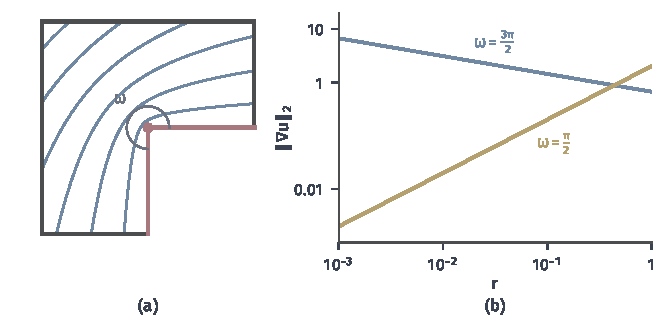
\includegraphics[width=112mm]{figures/06-differential-equations/02-partial-differential-equations/matplotlib/ellip-corner/figure.pdf}
  \caption{角点限制整体光滑性。(a)L形区域上$u=r^{2/3}\sin(2\theta/3)$的等值线，红色的两条边上$u=0$，它们在内角$\omega=3\pi/2$的顶点相交。(b)梯度大小随$r$的变化：$\omega=3\pi/2$时（蓝）$\frac23r^{-1/3}$在顶点爆炸，$\omega=\pi/2$的$r^2\sin2\theta$（黄）梯度$2r$在顶点趋于零。}
  \label{fig:ellip-corner}
\end{BookInlineFigure}

梯度的大小是$\frac23r^{-1/3}$，在顶点处趋于无穷，但其平方可积：
\[
 \int_0^1r^{-2/3}\,r\,\mathrm{d}r<\infty .
\]
所以$u\in H^1$，它是合法的弱解。二阶导数的大小是$r^{-4/3}$量级，平方的积分
\[
 \int_0^1r^{-8/3}\,r\,\mathrm{d}r
\]
发散，所以$u\notin H^2$。再取一个在顶点附近恒为$1$、支撑很小的光滑截断函数$\eta$，令$\tilde u=\eta u$。由乘积法则和$\Delta u=0$，
\[
 -\Delta\tilde u=-2\nabla\eta\cdot\nabla u-u\,\Delta\eta ,
\]
它只在$\eta$不是常数的地方非零，那里$u$光滑。所以$\tilde u$是光滑源项、全零边界值的问题的弱解，在顶点附近却与$u$相同，不属于$H^2$。

一般地，内角$\omega$对应的奇性是$r^{\pi/\omega}$。二阶导数的量级是$r^{\pi/\omega-2}$，平方可积当且仅当$\pi/\omega>1$，即$\omega<\pi$。内角超过$\pi$时奇性无法避免，这不是系数或数据的问题，而是几何本身的限制。

边界条件类型的切换也会产生奇性，哪怕边界本身是光滑的。在上半平面取$u=r^{1/2}\sin(\theta/2)$，它在正半轴$\theta=0$上满足$u=0$，在负半轴$\theta=\pi$上满足$\partial_\theta u=0$。切换点处的梯度量级是$r^{-1/2}$，同样不在$H^2$中。

把各种因素放在一起，可以这样理解：弱解的存在由能量和强制性决定，对光滑性没有要求；更高的光滑性是额外的收获，需要系数、源项和边界几何都配合，其中任何一个粗糙都会限制最终的结果。第~\ref{chap:pde-numerical-methods}章的有限元收敛阶，正是由这里的正则性决定的。
